\section{NMPC Planner}

	\begin{frame}
		\centering
		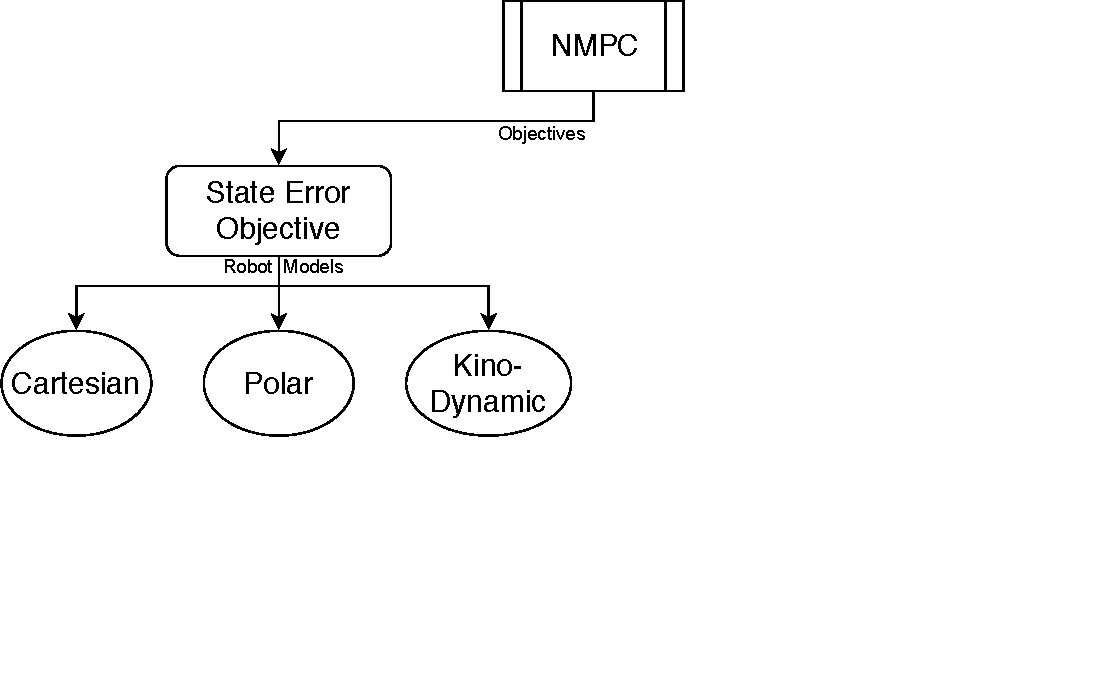
\includegraphics[scale=0.7]{pictures/mpc_planner_group/mpc_planner_8.pdf}
	\end{frame}

	\begin{frame}
		\frametitle{Robot Models Used}
		\begin{columns}[T]
			\begin{column}{0.45\textwidth}
				\onslide<2->{
				\begin{block}{Cartesian Co-ordinate Model}
					\[
					\begin{bmatrix}
						\dot{x} \\
						\dot{y} \\
						\dot{\theta}
					\end{bmatrix}
					=
					\begin{bmatrix}
						\cos(\theta) & 0 \\
						\sin(\theta) & 0 \\
						0 & 1
					\end{bmatrix}
					\begin{bmatrix}
						\upsilon \\
						\omega 
					\end{bmatrix}
					\]
				\end{block}
				}
				\onslide<3->{
				\begin{block}{Kino-dynamic Model}
					\[
					\begin{bmatrix}
						\dot{x} \\
						\dot{y} \\
						\dot{\theta} \\
						\dot{\upsilon} \\
						\dot{\omega}
					\end{bmatrix}
					=
					\begin{bmatrix}
						\cos(\theta) & 0 & 0 & 0 \\
						\sin(\theta) & 0 & 0 & 0 \\
						0 & 1 & 0 & 0 \\
						0 & 0 & 1 & 0 \\
						0 & 0 & 0 & 1
					\end{bmatrix}
					\begin{bmatrix}
						\upsilon \\
						\omega \\
						a \\
						\alpha
					\end{bmatrix}
					\]
				\end{block}
				}
			\end{column}
			\begin{column}{0.49\textwidth}
				\centering
				\onslide<1->{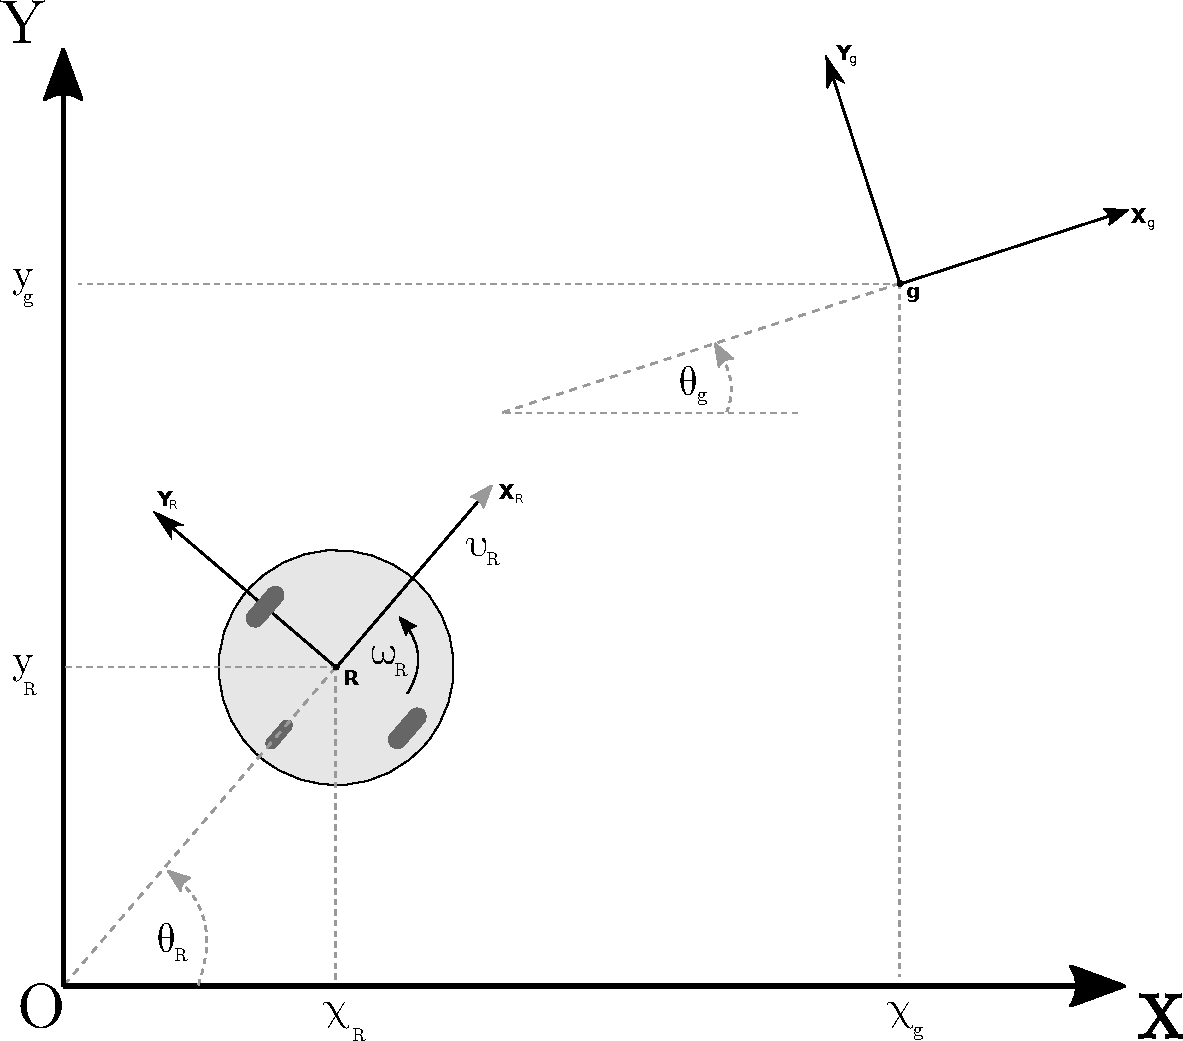
\includegraphics[scale=0.35]{pictures/robot_cart.pdf}}
			\end{column}
		\end{columns}
	\end{frame}

	\begin{frame}
		\frametitle{Robot Models Used}
		\begin{columns}[T]
			\begin{column}{0.45\textwidth}
				\onslide<2->{
				\begin{block}{Polar Co-ordinate Model}
					\begin{align*}
						\rho& = \sqrt{x^2+y^2} \\
						\phi& = \arctan2(y,x) \\
						\alpha&= \phi - \theta
					\end{align*}
				\end{block}
				}
			\end{column}
			\begin{column}{0.49\textwidth}
				\centering
				\onslide<1->{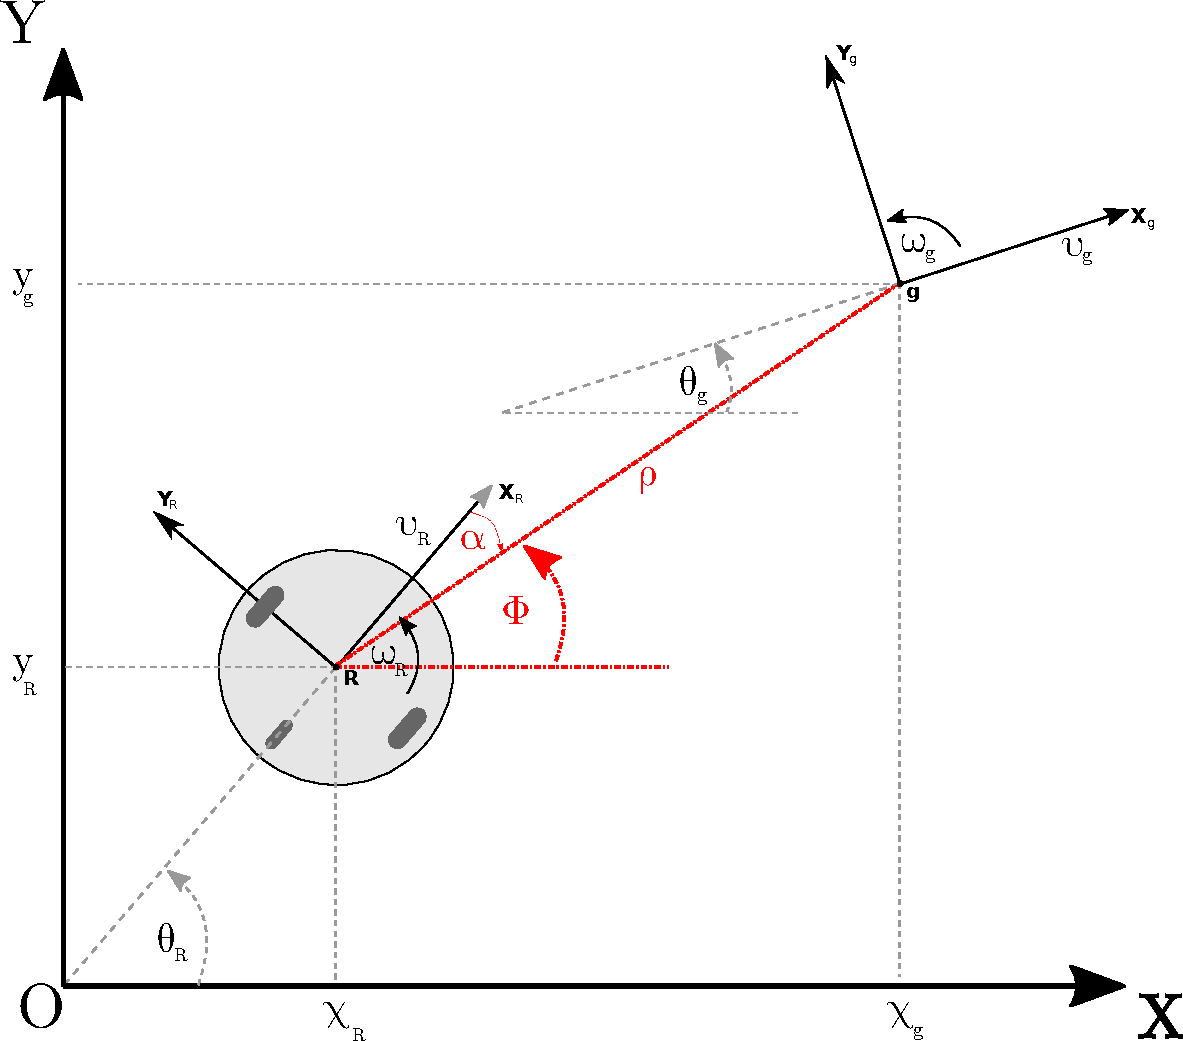
\includegraphics[scale=0.35]{pictures/robot_polar.pdf}}
			\end{column}
		\end{columns}
	\end{frame}

	\begin{frame}
		\frametitle{NMPC General Formulation}
		\begin{block}{NMPC Optimization Problem}
			\begin{align*}
				&\underset{\mathbf{X}^*,\mathbf{U}^*}{\text{min    }}
				\tikzmark{a9}J_{N_p}(\mathbf{x}_k) = \tikzmark{a10}V_f(\mathbf{x}_{k+N_p}) + \sum_{j=0}^{N_p-1}\tikzmark{a11}\ell (\mathbf{x}_{k + j},\mathbf{u}_{k + j}), \\
				&\quad \text{subject to:} \notag  \\
				&\quad\quad \tikzmark{a12}\mathbf{x}_{k+j+1} = \mathcal{F}(\mathbf{x}_{k+j},\mathbf{u}_{k+j}), & \forall\text{ } 0\leq j\leq N_p-1  \\ 
				&\quad\quad \tikzmark{a13}\mathbf{x}_{k+j} \in \mathbb{X}, & \forall \text{ }0\leq j\leq N_p \\
				&\quad\quad \tikzmark{a14}\mathbf{u}_{k+j} \in \mathbb{U}, & \forall \text{ }0\leq j\leq N_p-1 \\
				&\quad\quad \tikzmark{a15}\mathbf{d}_{\imath,k+j}  \geq \xi_o, & \forall\text{ } 0\leq j\leq N_p-1, \text{ }\forall\text{ } \imath \in I_s
			\end{align*}
		\end{block}
	
		\begin{tikzpicture}[overlay, remember picture]
			\coordinate (A9) at ($({pic cs:a9})+(1ex, 1ex)$);
			\coordinate (A10) at ($({pic cs:a10})+(1ex, 1ex)$);
			\coordinate (A11) at ($({pic cs:a11})+(1ex, 1ex)$);
			\coordinate (A12) at ($({pic cs:a12})+(0ex, 0.5ex)$);
			\coordinate (A13) at ($({pic cs:a13})+(0ex, 0.5ex)$);
			\coordinate (A14) at ($({pic cs:a14})+(0ex, 0.5ex)$);
			\coordinate (A15) at ($({pic cs:a15})+(1ex, -0.5ex)$);
			\pause
			\node [fit=(A9), baseline] (n9) {};
			\node[cyan, above of= n9, node distance = 3em] (t9_1) {\small cost};
			\node[cyan, above of= n9, node distance = 2em] (t9) {\small function};
			\draw [<-, cyan] (n9.north) to [below] (t9.south);
			\pause
			\node [fit=(A10), baseline] (n10) {};
			\node[cyan, above of= n10, node distance = 3em] (t10_1) {\small terminal};
			\node[cyan, above of= n10, node distance = 2em] (t10) {\small penalty};
			\draw [<-, cyan] (n10.north) to [below] (t10.south);
			\pause
			\node [fit=(A11), baseline] (n11) {};
			\node[cyan, above of= n11, node distance = 3em] (t11_1) {\small regulatory};
			\node[cyan, above of= n11, node distance = 2em] (t11) {\small term};
			\draw [<-, cyan] (n11.north) to [below] (t11.south);
			\pause
			\node [fit=(A12), baseline] (n12) {};
			\node[cyan, left of= n12, node distance = 4em] at (2,3) (t12) {\small model};
			\node[cyan, below of= t12, node distance = 1em] (t12_1) {\small constraints};
			\draw [<-, cyan] (n12.west) to [right] (t12.east);
			\pause
			\node [fit=(A13), baseline] (n13) {};
			\node[cyan, left of= n13, node distance = 4em] (t13) {\small state};
			\node[cyan, below of= t13, node distance = 1em] (t13_1) {\small boundries};
			\draw [<-, cyan] (n13.west) to [right] (t13.east);
			\pause
			\node [fit=(A14), baseline] (n14) {};
			\node[cyan, left of= n14, node distance = 4em] at (2,1) (t14) {\small input};
			\node[cyan, below of= t14, node distance = 1em] (t14_1) {\small boundries};
			\draw [<-, cyan] (n14.west) to [right] (t14.east);
			\pause
			\node [fit=(A15), baseline] (n15) {};
			\node[cyan, below of= n15, node distance = 3em] (t15_1) {\small static};
			\node[cyan, below of= n15, node distance = 2em] (t15) {\small obstacles};
			\draw [<-, cyan] (n15.south) to [above] (t15.north);
		\end{tikzpicture}
	\end{frame}
	
	\begin{frame}
		\frametitle{NMPC General Formulation}
		\begin{block}{Regulatory Terms (e.g., Cartesian coordinate)}
			\[
				\begin{aligned}
					\ell (\mathbf{x}_{k + j},\mathbf{u}_{k + j}) = \enspace
					\tikzmark{a1}
					(\mathbf{x}_{k + j} - \mathbf{x}_{ref})^T \enspace Q_1 \enspace (\mathbf{x}_{k + j} - \mathbf{x}_{ref})
					\tikzmark{a2}
					\enspace + \enspace
					\tikzmark{a3}
					\Delta\mathbf{u}_{k + j}^T \enspace R \enspace \Delta\mathbf{u}_{k + j}
					\tikzmark{a4}
					\enspace \tikzmark{a7}-\tikzmark{a8} \enspace
					\tikzmark{a5} 
					\sum_{i=0}^{I} \mathbf{d}_{i,k + j}^T \enspace Q_2 \enspace \mathbf{d}_{i,k + j}
					\tikzmark{a6}
				\end{aligned}
			\]
		\end{block}
		\vfill
		\vfill
		\vfill
		\begin{itemize}
			\item $\mathbf{d}_{i,k + j}$: distance between the robot and $i^{th}$ detected moving obstacle.
		\end{itemize}
		
		\begin{tikzpicture}[overlay, remember picture]
			\coordinate (A1) at ($({pic cs:a1})+(+0.1ex, 2ex)$);
			\coordinate (A2) at ($({pic cs:a2})+(-0.1ex,-0.5ex)$);
			\coordinate (A3) at ($({pic cs:a3})+(+0.1ex, 2ex)$);
			\coordinate (A4) at ($({pic cs:a4})+(-0.1ex,-0.5ex)$);
			\coordinate (A5) at ($({pic cs:a5})+(+0.1ex, 3.5ex)$);
			\coordinate (A6) at ($({pic cs:a6})+(-0.1ex,-2.5ex)$);
			\coordinate (A7) at ($({pic cs:a7})+(+1ex, 0.5ex)$);
			\coordinate (A8) at ($({pic cs:a8})+(-1ex, 0.5ex)$);
			\pause
			\node [fit=(A1)(A2), draw=tugreen, thick, rounded corners] (n1) {};
			\node[overlay, below of= n1, node distance = 6em] (t1) {State Error};
			\node[overlay, below of= n1, node distance = 7em] (t1_1) {Objective};
			\draw [thick, -latex, tugreen] (n1.south) to [above] (t1.north);
			\pause
			\node [fit=(A3)(A4), draw=tugreen, thick, rounded corners] (n2) {};
			\node[overlay, below of= n2, node distance = 6em] (t2) {Input Penealty};
			\node[overlay, below of= n2, node distance = 7em] (t2_1) {Objective};
			\draw [thick, -latex, tugreen] (n2.south) to [above] (t2.north);
			\pause
			\node [fit=(A5)(A6), draw=tugreen, thick, rounded corners] (n3) {};
			\node[overlay, below of= n3, node distance = 5.7em] (t3) {Dyn Obstacles};
			\node[overlay, below of= n3, node distance = 6.7em] (t3_1) {Objective};
			\draw [thick, -latex, tugreen] (n3.south) to [above] (t3.north);
			\pause
			\node [fit=(A7)(A8), draw=red, circle] (n4) {};
			\node[overlay, red, above of= n4, node distance = 8em] (t4) {Maximization};
			\draw [thick, -latex, red] (n4.north) to [below] (t4.south);
		\end{tikzpicture}
		
%		\tikz[baseline=(n1.base)]{
%			\node[draw=tugreen, ,thick, rounded corners, inner sep=5pt] 
%			(n1){$xfoz$};
%			\node[overlay, below of= n1, node distance = 6em] (t1) {State Error};
%			\draw [thick, -latex, tugreen] (n1.south) to [above] (t1.north);
%		}
	\end{frame}
	
	\begin{frame}
		\frametitle{Potential Collision Zone}
		\centering
		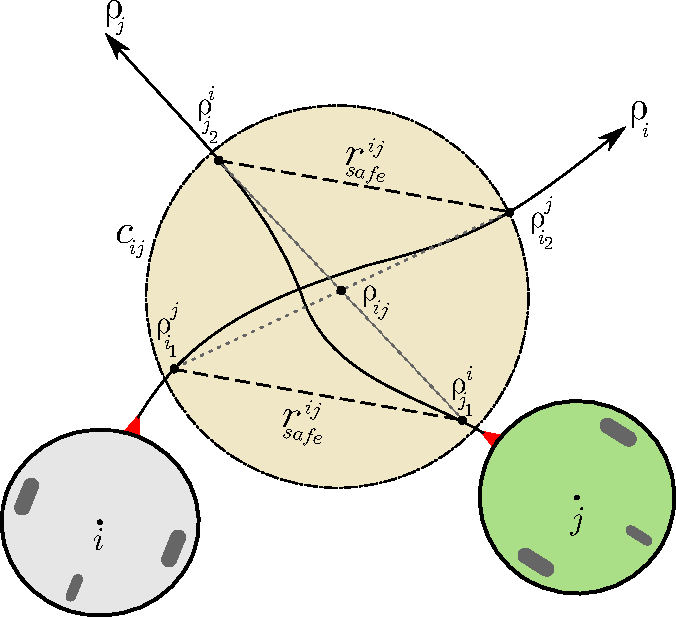
\includegraphics[scale=0.6]{pictures/robots_pot_coll.pdf}
	\end{frame}
	
	\begin{frame}
		\frametitle{Cartesian Coordinate Model Block Diagram}
		\begin{figure}[hbtp]
			\centering
			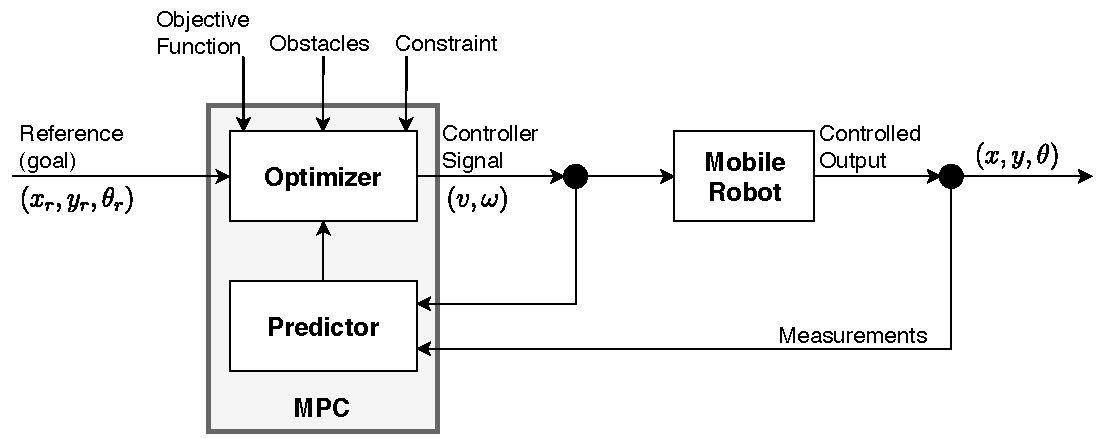
\includegraphics[scale=0.7]{pictures/block_diagram_cart.pdf}
			\caption{NMPC Control Loop (Cartesian coordinate Model)}
		\end{figure}
	\end{frame}

	\begin{frame}
		\frametitle{Polar Coordinate Model}
		\begin{block}{Regulatory Term}
			\parbox[c][4\baselineskip][t]{\textwidth}{
			\begin{align*}
				\ell_p (\vartheta_{k + j},\mathbf{u}_{k + j}) &= 
				\pmb{[} \ell_{p,1}(\cdot,\cdot) \enspace \ell_{p,2}(\cdot,\cdot) \enspace \ell_{p,3}(\cdot,\cdot) \pmb{]}
				\enspace
				\mathbf{Q_1} \enspace
				\begin{bmatrix}
					\ell_{p,1}(\cdot,\cdot) \\
					\ell_{p,2}(\cdot,\cdot) \\
					\ell_{p,3}(\cdot,\cdot)
				\end{bmatrix}
				+ \cdots
			\end{align*}
			}
		\end{block}
		Minimization of:
		\begin{itemize}
			\item Euclidean distance: $\ell_{p,1}(\cdot,\cdot) = \sqrt{(x_{k+j} - x_{ref})^2+(y_{k+j} - y_{ref})^2}$
			\item Heading towards goal: $\ell_{p,2}(\cdot,\cdot) = \Big(\theta_{k+j} - \arctan2\big((y_{k+j} - y_{ref}),(x_{k+j} - x_{ref})\big)\Big)^2$
			\item Reference orientation: $\ell_{p,3}(\cdot,\cdot) = (\theta_{k+j} - \theta_{ref})^2$
		\end{itemize}
	\end{frame}

	\begin{frame}
		\frametitle{Polar Coordinate Model Block Diagram}
		\begin{figure}[hbtp]
			\centering
			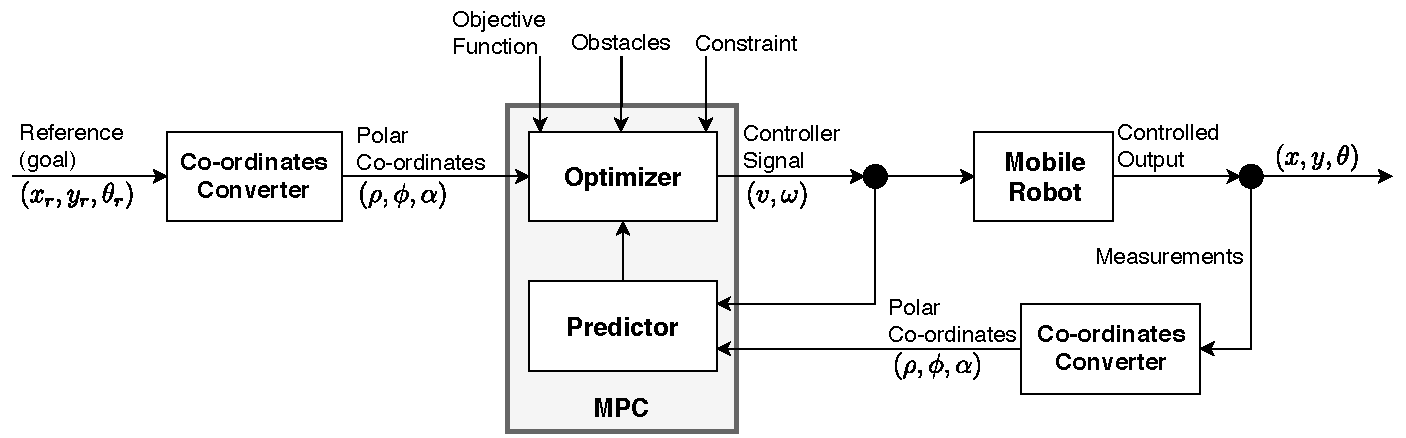
\includegraphics[scale=0.64]{pictures/block_diagram_polar.pdf}
			\caption{NMPC Control Loop (Polar coordinate Model)}
		\end{figure}
	\end{frame}

	\begin{frame}
		\frametitle{Kino-dynamic Model Block Diagram}
		\begin{figure}[hbtp]
			\centering
			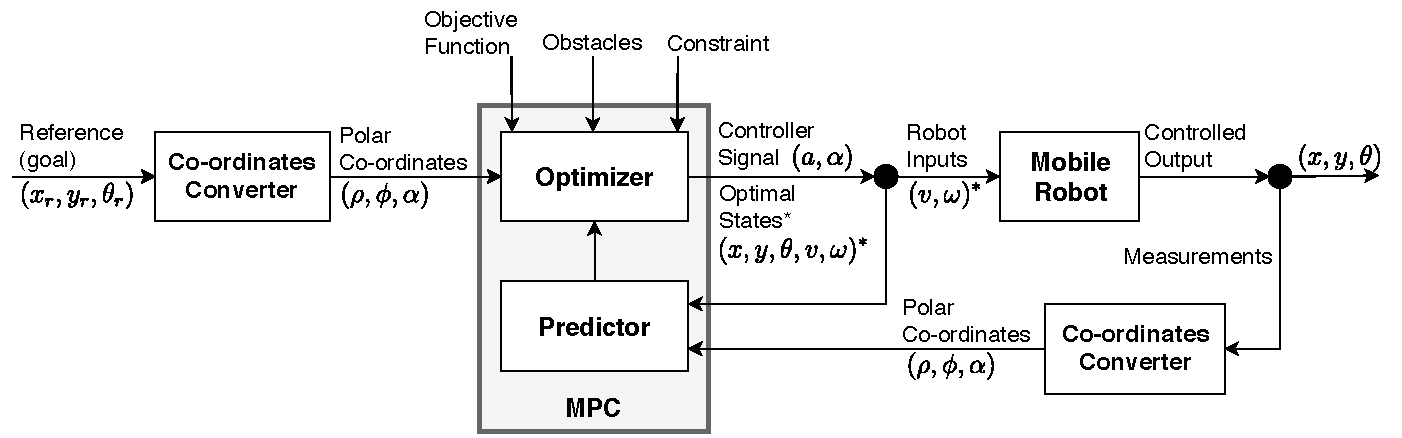
\includegraphics[scale=0.64]{pictures/block_diagram_kino.pdf}
			\caption{NMPC Control Loop (Kino-dynamic Model)}
		\end{figure}
	\end{frame}

	\begin{frame}
		\frametitle{NMPC with Switching Objective}
		\onslide<1->
		{
		\begin{block}{Optimization Problem}
			\parbox[c][3\baselineskip][t]{\textwidth}{
				\begin{align*}
				\underset{\vartheta^*,\mathbf{U}^*}{\text{min    }}
				J_{N_p}(\vartheta_k) = (1 - \tikzmark{a16}\beta_2 - \tikzmark{a17}\beta_3) \times J_1 + 
				\tikzmark{a18}\beta_2 \times J_2 - \tikzmark{a19}\beta_3 \times J_3
				\end{align*}
			}
		\end{block}
		}
		\onslide<3->
		{Objectives:}
		\begin{itemize}
			\onslide<4->
			{\item $J_1 = \ell_{p,1}(\cdot,\cdot)$}
			\onslide<5->
			{\item $J_2 = w_2 \times J_1 + J_4$}
			\onslide<6->
			{\item $J_3 = w_3 \times J_1 + J_5$ \\ [1cm]}
		\end{itemize}
		\onslide<7->
		{
		\[
		J_{N_p}(\vartheta_k) = 
		\begin{cases}
			\beta_2 = 0, \enspace \beta_3 = 1, 				& \text{if a dynaminc obstacle is detected} \\
			\beta_2 = 1, \enspace \beta_3 = 0, 				& \text{else, if the robot is near the goal} \\
			\beta_2 = 0, \enspace \beta_3 = 0, 				& \text{otherwise} 
		\end{cases}
		\]
		}
		\begin{tikzpicture}[overlay, remember picture]
			\coordinate (A16) at ($({pic cs:a16})+(1ex, 0.5ex)$);
			\coordinate (A17) at ($({pic cs:a17})+(1ex, 0.5ex)$);
			\coordinate (A18) at ($({pic cs:a18})+(1ex, 0.5ex)$);
			\coordinate (A19) at ($({pic cs:a19})+(1ex, 0.5ex)$);
			\onslide<2->{
			\node [fit=(A16), draw=tugreen, circle, thick, inner sep=4.5pt] (n16) {};
			\node [fit=(A17), draw=tugreen, circle, thick, inner sep=4.5pt] (n17) {};
			\node [fit=(A18), draw=tugreen, circle, thick, inner sep=4.5pt] (n18) {};
			\node [fit=(A19), draw=tugreen, circle, thick, inner sep=4.5pt] (n19) {};
			\node[overlay, below of= n16, node distance = 4em] at (8.5,5) (t16) {Binary};
			\node[overlay, below of= t16, node distance = 1em] (t16_1) {Multipliers};
			\draw [thick, -latex, tugreen] (n16.south) to [above] (t16.north);
			\draw [thick, -latex, tugreen] (n17.south) to [above] (t16.north);
			\draw [thick, -latex, tugreen] (n18.south) to [above] (t16.north);
			\draw [thick, -latex, tugreen] (n19.south) to [above] (t16.north);
			}
		\end{tikzpicture}
	\end{frame}

	\begin{frame}
		\frametitle{NMPC with Switching Objective Block Diagram}
		\begin{figure}[hbtp]
			\centering
			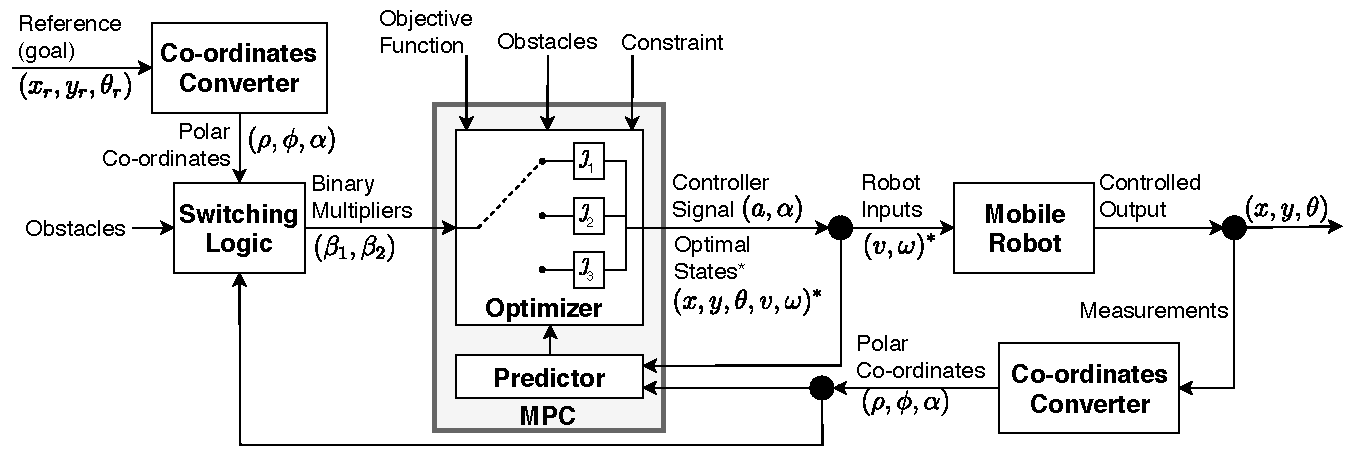
\includegraphics[scale=0.65]{pictures/block_diagram_polar_switch_1.pdf}
			\caption{NMPC Control Loop with Switching Objective}
		\end{figure}
	\end{frame}


